
\chapter{The 2-Dimensional Problem}\label{chap11}

\section{Introduction}\label{chap11:sec11.1}

We now\pageoriginale consider the approximation of the equations of
fluid dynamics in 2 dimensions, in the plane symmetric case. Once
again we have two coordinate systems-the Lagrangian coordinates
$(a,b)$ and the Eulerian coordinates $(x,y)$. These are connected by
the transformation 
\begin{equation*}
x = x(a, b , t), \;  y = y (a,b,t)\tag{11.1}\label{eq11.1}
\end{equation*}
where $x(a,b,t)$ and $y(a,b,t)$ are the coordinates at time $t$ of the
fluid particle located at $(a,b)$ at time $t =0$. We denote by $J$ the
Jacobian of the transformation (\ref{eq11.1}).  One defines the time
derivative $\dfrac{Df}{Dt}$ (so called ``particular derivative'') by  
\begin{equation*}
\frac{Df}{Dt} = \frac{\partial f}{\partial t} + u \frac{\partial
  f}{\partial x} + v \frac{\partial t}{\partial y}
\tag{11.2}\label{eq11.2} 
\end{equation*}
where $u$ and $v$ are the velocity components. The Lagrangian form of
the equation of motion is as follows: 

\medskip
\noindent{\textbf{Conservation of mass:}}
\begin{equation*}
\frac{D\rho}{Dt} + \rho div. \; \vec{u} = 0, \; \vec{u} = (u,v) \tag{11.3}\label{eq11.3}
\end{equation*}
or, equivalently,
\begin{equation*}
\frac{D}{Dt} (\rho J) = 0. \tag*{$(11.3')$}\label{eq11.3'}
\end{equation*}

\medskip
\noindent{\textbf{Conservation of momentum.}}
\begin{equation*}
\left. 
\begin{aligned}
{\rm (i)} & \qquad \rho \frac{Du}{Dt} + \frac{\partial}{\partial x} (p+q) = 0\\
{\rm (ii)} & \qquad \rho \frac{Du}{Dt} + \frac{\partial}{\partial y} (p+q) = 0.\\
\end{aligned}
\right\}
\tag{11.4}\label{eq11.4}
\end{equation*}
where $q$ is the pseudo-viscous term given by 
\begin{equation*}
q = \sigma (-div. \vec{u})\tag{11.5}\label{eq11.5}
\end{equation*}\pageoriginale 
with 
\begin{equation*}
\sigma = 
\begin{cases}
0, \text{ if } div \vec{u} > 0\\
\rho \ell^2 |div \vec{u}|, \text{ if } div \vec{u} < 0. 
\end{cases}\tag{11.6}\label{eq11.6}
\end{equation*}

\medskip
\noindent{\textbf{Conservation of energy.}}
\begin{equation*}
\frac{D\epsilon}{Dt} + (p+q) \frac{D}{Dt} (\frac{1}{\rho}) = 0. 
\tag{11.7}\label{eq11.7}
\end{equation*}

One also has the equation of state 
\begin{equation*}
\epsilon = f(p, \rho).\tag{11.8}\label{eq11.8}
\end{equation*}

\begin{remark}\label{chap11:rem11.1}
One reiterates our comments of Sec. \ref{chap1:sec1.5}, regarding the
Lagrangian form of the equations. In the equations above
$\dfrac{\partial}{\partial x} $ and $\dfrac{\partial}{\partial y}$
must be expressed in terms of derivatives w.r.t. $a$ and $b$ via the
Jacobian $J$.  
\end{remark}

\section{The weak form}\label{chap11:sec11.2}

We use the finite element method to discretise the equations of hydrodynamics w.r.t. the space variables. For this we need to write these equations in the weak form.

Let $\Omega$ be the domain of consideration and $\partial \Omega$ its boundary. Let $\vec{\nu} = (\nu_x, \nu_y)$ be the unit outer normal along $\partial \Omega$.

To write the equations in the weak form, we multiply our equations by suitable test-functions and integrate over $\Omega$. We write equations (\ref{eq11.3}) in the form 
\begin{equation*}
\int\limits_\Omega \left(\frac{D\rho}{Dt} + \rho div. \vec{u}\right) \varphi dx
\; dy =0. \tag{11.9}\label{eq11.9} 
\end{equation*}
for all suitable $\varphi$.

If $(\varphi, \psi)$ is a test-vector, then an multiplying
(\ref{eq11.4}) (i) by $\varphi$ and (\ref{eq11.4}) (ii) by $\psi$ and
integrating by parts, we get the weak form: 
\begin{equation*}
\left. 
\begin{aligned}
{\rm (i)} & \qquad \int\limits_\Omega \rho\frac{Du}{Dt} \varphi dx \;
dy + \int\limits_{\partial \Omega} p \varphi \nu_x ds -
\int\limits_\Omega p \frac{\partial \varphi}{\partial x} dx \; dy =
0\\ 
{\rm (ii)} & \qquad \int\limits_\Omega \rho \frac{Dv}{Dt} \psi dx \;
dy + \int\limits_{\partial\Omega} p \psi \nu_y \; ds -
\int\limits_\Omega p \frac{\partial \psi}{\partial y} dx \; dy = 0.\\ 
\end{aligned}
\right\}
\tag{11.10}\label{eq11.10}
\end{equation*}\pageoriginale 
for all suitable $\varphi$ and $\psi$. Thus we have got rid of all the derivatives of $p$ in (\ref{eq11.4}). Since the third equation viz., (\ref{eq11.7}) does not involve derivatives w.r.t. space variables we keep it as it is.

From these equations it is clear that it suffices to take $\rho$, $p$, $\epsilon \in L^2 (\Omega)$ while we need $x,y,u, v,\varphi, \psi \in H^1 (\Omega)$. We shall use the finite element method with quadrilateral elements and trial functions which are piecewise polynomials. Thus we need to have these trial functions continuous across the inter element boundaries (Cf. Ciarlet \cite{key6}) in order that these functions may be in $H^1(\Omega)$.

We now proceed to describe the simplest element known.

\section{An isoparametric quadrilateral element}\label{chap11:sec11.3}
Let us assume that the domain $\Omega$ is such that it can be subdivided into quadrilaterals. Since we only need $\rho$, $p$, $\epsilon \in L^2 (\Omega)$, one can take as trial functions the space $V_\circ$ of piecewise constant (which are, in particular, discontinuous) functions. Thus if $\chi_Q$ is the characteristic function of the quadrilateral $Q$, then one can write
$$
V_\circ = \left\{ \sum\limits_Q \alpha_Q \chi_Q \mid \alpha_Q = \alpha_Q (t), \text{ a constant w.r.t. $a$ and $b$}\right\} \subset L^2 (\Omega).
$$

Now to achieve a space of approximants contained in $H^1 (\Omega)$, as already mentioned, we use continuous piecewise polynomials.

This is most easily achieved if we can define these functions in each quadrilateral $Q$ in such a way so that they depend only on their values at the four nodes of $Q$, and along each boundary their restriction is a linear interpolation of the values at the end vertices. Then, obviously, given two adjacent elements\pageoriginale $Q$ and $Q^1$, if the values of a piecewise polynomial, $f$, are prescribed at the nodes then the restriction of $f$ to that common edge from both $Q$ and $Q^1$ will be the same and hence continuity is established.

If $Q$ is a rectangle whose sides are parallel to the axes (say. the
unit square) then the definition of such polynomials is easy
(Fig. \ref{c11:fig11.1}). 

\begin{figure}[H]
\centering
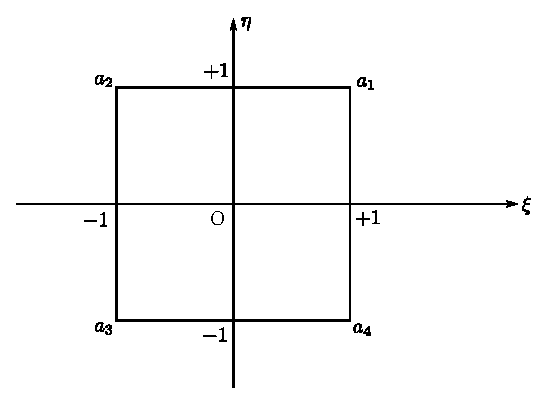
\includegraphics{figures/fig52-11.1.eps}
\caption{}\label{c11:fig11.1}
\end{figure}

We define the space of polynomials to be
$$
Q_1 = \left\{ p(\xi, \eta) \mid p(\xi, \eta) = a + b\xi + c \eta + d
\xi \eta\right\}.  
$$

Then restricted to each side, $p(\xi, \eta)$ is a polynomial of degree
$\leq 1$ either in $\xi$ or in $\eta$ alone. Further it is linearly
interpolated on each edge between the values at the end-points. In
fact one can give a basis for $Q_1$ by four polynomials $\ell_i
(i=1,2,3,4)$ such that $\ell_i \in Q_1$ and $\ell_i$ takes the value 1
at the vertex $a_i$ and zero at the other vertices. Thus  
\begin{equation*}
\left.
\begin{aligned}
\ell_1 (\xi, \eta) & = \frac{1}{4} (1+\xi) (1+\eta) \quad \\
\ell_2 (\xi, \eta) & = \frac{1}{4} (1-\xi) (1+\eta) \quad \\
\ell_3 (\xi, \eta) & = \frac{1}{4} (1-\xi) (1-\eta) \quad \\
\ell_4 (\xi, \eta) & = \frac{1}{4} (1+\xi) (1-\eta). \quad 
\end{aligned}
\right\}\tag{11.11}\label{eq11.11}
\end{equation*}

If\pageoriginale $p \in Q_1$, one has
$$
p(\xi, \eta) = \sum\limits^4_{i+1} p(a_i) \ell_i (\xi, \eta).
$$
Thus $Q_1$ has all the properties we need.

Let us go to a general quadrilateral with vertices $A_1, A_2, A_3$ and $A_4$ in the $(a,b)$-plane.

\begin{figure}[H]
\centering
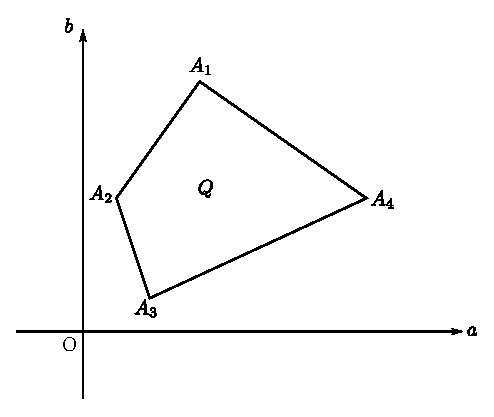
\includegraphics{figures/fig52-11.2.eps}
\caption{}\label{c11:fig11.2}
\end{figure}


We now define a transformation
\begin{equation*}
\left. 
\begin{aligned}
a(\xi, \eta) & = \sum\limits^4_{i=1} a_i \ell_i (\xi, \eta)\\
b(\xi, \eta) & = \sum\limits^4_{i=1} b_i \ell_i (\xi, \eta)
\end{aligned}
\right\}
\tag{11.12}\label{eq11.12}
\end{equation*}
so that $a_1 \mapsto A_1$, $a_2 \mapsto A_2$, $a_3 \mapsto A_3$ and
$a_4 \mapsto A_4$. It is routine checking to see that the four edges
of the square map linearly into the corresponding edges of the
quadrilateral, i.e. if $0 \leq \lambda \leq 1$, then the point $\lambda
a_i+(1-\lambda) a_{i+1} $ maps to the point $\lambda A_i + (1-\lambda)
A_{i+1}$. Further, the transformation can be inverted. i.e. for every
point $(a,b) \in Q$, there exists a unique point $(\xi, \eta)$ in the
unit square which maps into $(a,b)$ under the transformation
(\ref{eq11.12}). We use this correspondence to define a space $V_Q$ of
polynomials over $Q$: 
\begin{equation*}
V_Q = \{u (a,b) \mid u(a,b) = \sum\limits^4_{i=1} u(A_i) \ell_i
(\xi, \eta)\}. \tag{11.13}\label{eq11.13} 
\end{equation*}\pageoriginale

Then it is easy to see that $u$ is completely determined by its values on the nodes and that on each boundary it is a linear interpolation of the values at the end-points. 

Now given a subdivision of $\Omega$ into quadrilaterals, we define $V_1$ by 
\begin{equation*}
V_1 = \{u \mid u \mid Q \in V_Q\}. \tag{11.14}\label{eq11.14}
\end{equation*}

Then $V_1$ satisfies the continuity condition and hence is a subspace
of $H^1(\Omega)$. Also every function in $V_1$ is completely
described by its values at all the nodes. Indeed if we number all the
nodes of the subdivision suitably and if $\varphi_i$ is that function
of $V_1$ whose value at the $i^{\rm th}$ node is 1 and it  takes the
value 0 at other nodes, for $1 \leq i \leq I$, then such functions
form a basis for $V_1$. Every function $u \in V_1$ may be written as  
\begin{equation*}
u = \sum\limits^I_{i =1} u_i \varphi_i
\tag{11.15}\label{eq11.15}
\end{equation*}
where $u_i = u_i(t)$ is the value of $u$ at the i-th node.

Another important property of the functions $\varphi_i$ is, that $\varphi_i$ is non-zero only on atmost  four quadrilaterals of which the $i^{\rm th}$ node is a vertex. (We will come to the question of boundary nodes later).

Such finite elements as described in this section are called
isoparametric because we use the {\em same} types of functions both
for the space of approximants as well as for the transformations from
the unit square. (See Ciarlet and Raviart \cite{key7} for a complete
discussion on isoparametric finite elements). 

\section{Discretization of the equations}\label{chap11:sec11.4}

We now\pageoriginale discretise the weak forms of the equations. Thus
we substitute in the equations (\ref{eq11.9}), (\ref{eq11.10}) and
(\ref{eq11.7}) the trial functions and look for solutions in spaces of
these trial functions. Thus we take $p, \rho, \epsilon \in V_\circ$
and $u,v,x,y, \varphi, \psi \in V_1$ and demand that the equations
(\ref{eq11.10}) are satisfied for all $\varphi, \psi \in V_1$ and
(\ref{eq11.9}) for all $\chi_Q$. Of course, it is enough to satisfy
(\ref{eq11.10}) for the basis functions $\varphi_i$. In order to make
these statements precise and to obtain the discrete equations, we
first write  
\begin{equation*}
\left. 
\begin{aligned}
\rho & = \sum\limits_Q \rho_Q(t) \chi_Q, \; \epsilon = \sum\limits_Q \epsilon_Q (t) \chi_Q\\
p & = \sum\limits_Q p_Q(t) \chi_Q, \; u = \sum\limits^I_{i=1} u_i (t) \varphi_i, \; v = \sum\limits^I_{i=1} v_i (t) \varphi_i
\end{aligned}
\right\}
\tag{11.16}\label{eq11.16}
\end{equation*}
 where the nodes are numbered from 1 to $I$. Now equation
 (\ref{eq11.9}) becomes 
$$
\int\limits_\Omega \left(\frac{D\rho}{Dt} + \rho div \vec{u}\right)
\chi_Q dx \; dy = 0 \text{ for all } Q.  
$$
or 
$$
\int\limits_Q \left(\frac{D\rho}{Dt} + \rho div \vec{u}\right) dx \; dy = 0
\text{ for all } Q.  
$$
Using (\ref{eq11.16}) we get (by setting $S_Q$ to be the area of the
quadrilateral $Q$), the discretization of (\ref{eq11.9}) w.r.t. the
space variables as  
\begin{equation*}
S_Q \frac{D\rho_Q}{Dt} + \rho_Q \sum\limits_i u_i \int\limits_Q
\frac{\partial \varphi_i}{\partial x} dx \; dy + \rho_Q \sum\limits_i
v_i \int\limits_Q \frac{\partial \varphi_i}{\partial y} dx \; dy =  0
\tag{11.17}\label{eq11.17} 
\end{equation*}
for all $Q$.

Since in the equation (\ref{eq11.7}) everything is constant w.r.t. the
space variables. we get  
\begin{equation*}
  \frac{D\epsilon_Q}{Dt} + \left(p_Q \frac{D}{Dt}\right)
  \left(\frac{1}{\rho_Q}\right) = 0 
  \text{ for all } Q.  \tag{11.18}\label{eq11.18} 
\end{equation*}

We now show how to discretise (\ref{eq11.10}) (i). (The method for
(\ref{eq11.10}) (ii) is identical).  

Substituting\pageoriginale in (\ref{eq11.10}) (i) from (\ref{eq11.16}), we get
\begin{equation*}
\sum\limits_j \frac{Du_j}{Dt} \int\limits_\Omega \rho \varphi_j \varphi_i dx \; dy + \int\limits_{\partial \Omega} p \varphi_i \nu_x ds - \sum\limits_Q p_Q \int\limits_\Omega \chi_Q  \frac{\partial \varphi_i}{\partial x} dx \; dy = 0
\tag{11.19}\label{eq11.19}
\end{equation*}
for all $1\leq i \leq I$.

Using the fact that $\rho J = \rho_\circ$, we get
\begin{align*}
\sum\limits_j \frac{Du_j}{Dt} \int\limits_\Omega \rho_\circ \varphi_i \varphi_j da \; db & + \int\limits_{\partial \Omega} p \varphi_i \nu_x ds - \sum\limits_Q p_Q \int\limits_Q \frac{\partial \varphi_i}{\partial x} dx \; dy \tag{11.20}\label{eq11.20}\\
& = 0, \; 1 \leq i \leq I. 
\end{align*}

We see that the last term in (\ref{eq11.20}), which is similar to the last terms of (\ref{eq11.17}), will be non-zero only if the $i^{\rm th}$ node is a vertex of $Q$. Thus for every $i$, the last term expounds into at most four non-zero terms.

The middle term of (\ref{eq11.20}) survives only if $\varphi_i$ corresponds to a boundary node. We will turn to the question of boundary nodes in Sec. \ref{chap11:sec11.5}. 

Coming to the first term we see that $\varphi_i \varphi_j$ is non-zero only if $i$ and $j$ are vertices of the same quadrilateral. Thus the matrix $\int\limits_\Omega \rho_\circ \varphi_i \varphi_j da \; db$ has got at most 9 non-zero terms in each row. However in solving a numerical scheme inverting such a matrix is still expensive. So we replace this term by an approximation which yields a diagonal matrix.

We set 
\begin{equation*}
\int\limits_Q f \rho_\circ da \; db \sim \sum\limits^4_{k=1} f(A_k)
\alpha_k \int\limits_Q \rho_\circ da \; db \tag{11.21}\label{eq11.21} 
\end{equation*}
where $\{A_k\}^4_{k=1}$ are the four nodes of the quadrilateral $Q$. We define the $\alpha_k$ so that on replacing $f$ by the basis functions corresponding to the vertices of $Q$, the relation (\ref{eq11.21}) is an equality. Thus if $\varphi^k$ is the basis function corresponding to $A_k$, we have 
\begin{equation*}
\alpha_k = \frac{\int\limits_Q \varphi^k \rho_\circ da \; db}{\int\limits_Q \rho_\circ da \; db}. \tag{11.22}\label{eq11.22}
\end{equation*}\pageoriginale
We now have 
$$
\int\limits_Q \varphi_i \varphi_j \rho_\circ da db \sim
\sum\limits^4_{i=1} (\varphi_j \varphi_i) (A_k) \alpha_k \int\limits_Q
\rho_\circ da \; db.  
$$
The left-hand-side terms will be non-zero only if $i = j$ and $\varphi_i = \varphi^k$, the function which takes the value 1 at the node $A_k$.

Now to get the matrix in the coefficient of $\dfrac{DU}{Dt}$ where\break
$U^T =(u_1, \ldots, u_I)$ we compute it over each $Q$ and assemble
these together to get a diagonal matrix $M$. 

Thus in case we do not have the boundary term, the discretization of (\ref{eq11.10}) (i) reads as 
\begin{equation*}
M \frac{DU}{Dt} - A^T P = 0, \tag{11.23}\label{eq11.23}
\end{equation*}
where, if we number the quadrilaterals by $Q_1, \ldots, Q_N$, $P^T =
(p_{Q_1}, \ldots\break p_{Q_N})$ and $A^T$ is the $I\times N$ matrix whose
element in the $i^{\rm th}$ row and $n^{\rm th}$ column is  
$$
\int\limits_{Q_n} \frac{\partial \varphi_i}{\partial x} dx \; dy.
$$
Similarly, if $B^T$ is the matrix of order $I \times N$ whose $(i,n)$th-element is 
$$
\int\limits_{Q_n} \frac{\partial \varphi_i}{\partial y} dx \; dy, 
$$
the discretization of (\ref{eq11.10}) (ii) is 
\begin{equation*}
M \frac{DV}{Dt} - B^T P = 0. \tag{11.24}\label{eq11.24}
\end{equation*}

\section{The Boundary terms}\label{chap11:sec11.5}

Let us assume that $\Omega$ is a bounded domain. One essentially encounters two types of boundary conditions. viz., (i) with $p$ prescribed on the\pageoriginale boundary or (ii) with the normal velocity $\vec{u} \cdot \vec{\nu}$ prescribed on the boundary. Note that we impose only one boundary condition and not one each on both $u$ and $v$ as would be the case for a viscous fluid.

In the first case where $p$ is given, one has no problem with the term
$\int\limits_{\partial \Omega} p \varphi_i \nu_x ds$ of the equation
(\ref{eq11.20}).

Let us come to the second case. Let us assume that $\vec{u} \cdot
\vec{\gamma} = g$ is given. We now define a new unknown $p_{s}$, the
pressure on the boundary. We choose this $p_s$ to be approximated by
trial functions in the same space $H$. For example, $H$ could be the
space $H_\circ$ of piecewise constants on the boundary or $H_1$, the
space of continuous piecewise linear functions on the boundary, where,
by the work ``piecewise'' we mean w.r.t. the subdivision of the
boundary induced by the subdivision of $\Omega$ itself. Let $\{\chi_k
\}$ be a basis for $H$. Then we write 
$$
\int\limits_{\partial \Omega} (\vec{u} \cdot \vec{\nu} - g) \chi_k ds = 0 \text{ for all } k. 
$$
This expands as 
\begin{equation*}
\sum\limits_i \int\limits_{\partial \Omega} (u_i \varphi_i \nu_x + v_i \varphi_i \nu_y -g) \chi_k ds = 0, \tag{11.25}\label{eq11.25}
\end{equation*}
for each $k$ and this gives us  $K$ equations where $K$ is the dimension of $H$.

Also writing 
\begin{equation*}
p_s = \sum\limits^k_{k=1} (p_s)_k \chi_k, 
\tag{11.26}\label{eq11.26}
\end{equation*}
we substitute in (\ref{eq11.20}) to get the equations 
\begin{equation*}
\left. 
\begin{aligned}
M \frac{DU}{Dt} - A^T P + C P_S = 0 \quad \\
M \frac{DV}{Dt} - B^T P + D P_S = 0.
\end{aligned}
\right\}
\tag{11.27}\label{eq11.27}
\end{equation*}
where $P_S$ has as its components the $(p_s)_k$ indexed by $k$. 

One also\pageoriginale checks easily that (\ref{eq11.25}) takes the form 
\begin{equation*}
C^T U + D^T V  - G = 0\tag{11.28}\label{eq11.28}
\end{equation*}
where $G$ is a known vector. 

\section{Time discretization}\label{chap11:sec11.6}

As regards the time discretization, we evaluate $U,V$ at $(n+\frac{1}{2}) \Delta t$ and $p, \rho, \epsilon$ at time $n \Delta t$. For instance, equation \ref{eq11.3'} can be discretized by 
\begin{equation*}
\rho^{n+1}_Q \int\limits_Q J^{n+1} da \; db = \rho^n _Q \int\limits_Q J^n da \; db 
\tag{11.29}\label{eq11.29}
\end{equation*}
for all $Q$. 

The equation (\ref{eq11.7}) can be discretized exactly as in the
1 - dimensional case. The discretization for the momentum equations
involves the details described before. For instance, in the case of
the boundary pressure being zero one has  
\begin{equation*}
\left. 
\begin{aligned}
& M  \frac{U^{n+\frac{1}{2}} - U^{n-\frac{1}{2}}}{\Delta t} - A^T P^n = 0 \quad \\
& M  \frac{V^{n+\frac{1}{2}} - V^{n-\frac{1}{2}}}{\Delta t} - B^T P^n = 0. \quad \\
\end{aligned}
\right\} \tag{11.30}\label{eq11.30}
\end{equation*}

\section{Stability Criteria}\label{chap11:sec11.7}

We now sketch the procedure to get heuristic stability criteria.

Let us assume that (\ref{eq11.7}) and (\ref{eq11.8}) together can be
integrated to give $p$ as a function of $\rho$. Let us also have  
\begin{equation*}
\frac{\partial p}{\partial \rho} = \ob{C}^2,\tag{11.31}\label{eq11.31}
\end{equation*}
by linearising about some constant state defined by $(\bar{c},
\bar{\rho})$. Then (\ref{eq11.3}) gives  
\begin{equation*}
\frac{1}{\bar{\rho} \bar{c}^2} \frac{Dp}{Dt} + div \vec{u} = 0
\tag{11.32}\label{eq11.32}
\end{equation*}\pageoriginale 
where $\vec{u} = (u,v)$. Also the equations (\ref{eq11.4}) give 
\begin{equation*}
\bar{\rho} \frac{D\bar{u}}{Dt} + \text{ grad. } (p+q) = 0. 
\tag{11.33}\label{eq11.33}
\end{equation*}

Locally the derivatives in $t$ and in $x, y$ commute and hence one
gets from (\ref{eq11.32}) and (\ref{eq11.33}) 
\begin{equation*}
\frac{1}{\bar{c}^2} \frac{D^2 p}{Dt^2} - div \text{ grad. } (p+q)  = 0
\tag{11.34}\label{eq11.34}
\end{equation*}
where by (\ref{eq11.3}) and (\ref{eq11.5})
\begin{equation*}
q = \frac{\sigma}{\rho}  \frac{D\rho}{Dt} = \frac{\sigma}{\rho \bar{c}^2} \frac{Dp}{Dt} \tag{11.35}\label{eq11.35}
\end{equation*}

We imitate this procedure in the discrete case. One gets a discretization of (\ref{eq11.34}) from those of (\ref{eq11.3}) and (\ref{eq11.4}) and then studies the stability conditions. Now that we have div grad, which is nothing but the Laplacian, we are in a situation similar to that of the wave equation.

Let us assume that we do not have the surface pressure.

Proceeding as we did in Sec. \ref{chap11:sec11.4}, we get the discretization of (\ref{eq11.32}) as 
\begin{equation*}
\mathbb{N} \frac{P^{n+1} - P^n}{\Delta t} + A U^{n+\frac{1}{2}} + BV^{n+\frac{1}{2}} = 0
\tag{11.36}\label{eq11.36}
\end{equation*}
for all $n$ where $A, B$ are defined as in Sec. \ref{chap11:sec11.4} and the matrix $\mathbb{N}$ is an $(N \times N)$ matrix defined by
\begin{equation*}
N_Q = \frac{M_Q}{\rho^2_Q C^2_Q}\tag{11.37}\label{eq11.37}
\end{equation*}
where the suffix $Q$ denotes the diagonal element of $\mathbb{N}$ corresponding to the quadrilateral $Q$ and $M_Q$ is given by 
\begin{equation*}
M_Q = \int\limits_Q \rho_\circ da \; db. \tag{11.38}\label{eq11.38}
\end{equation*}\pageoriginale 
The discretization of (\ref{eq11.38}) gives 
\begin{equation*}
\left. 
\begin{aligned}
{\rm (i)} & \qquad M \frac{U^{n+\frac{1}{2}} - U^{n-\frac{1}{2}}}{\Delta t}  - A^T \left[ P^n + \sum \cdot \frac{P^n - P^{n-1}}{\Delta t} \right] =0 \quad \\
{\rm (ii)} & \qquad M \frac{V^{n+\frac{1}{2}} - V^{n-\frac{1}{2}}}{\Delta t}  - B^T \left[ P^n + \sum \cdot \frac{P^n - P^{n-1 }}{\Delta t} \right] = 0 \quad\\
\end{aligned}
\right\}
\tag{11.39}\label{eq11.39}
\end{equation*}
where $M$ is the diagonal matrix of Sec. \ref{chap11:sec11.4} and $\sum$ is a $N \times N$ diagonal matrix whose diagonal element corresponding to the quadrilateral $Q$ is given by 
\begin{equation*}
\sum_Q = \frac{\sigma_Q}{\rho_Q C^2_Q}
\tag{11.40}\label{eq11.40}
\end{equation*}

Now (\ref{eq11.39}) (i) and (ii) give 
\begin{equation*}
\left.
\begin{aligned}
{\rm (i)} & \qquad A \frac{(U^{n+\frac{1}{2}} - U^{n - \frac{1}{2}})}{\Delta t }  = A M^{-1} A^T \left[ P^n + \sum \frac{P^n- P^{n-1}}{\Delta t} \right]\\
{\rm (ii)} & \qquad B \frac{(V^{n+\frac{1}{2}} - V^{n - \frac{1}{2}})}{\Delta t }  = B M^{-1} B^T \left[ P^n + \sum \frac{P^n- P^{n-1}}{\Delta t} \right]\\
\end{aligned}
\right\}
\tag{11.41}\label{eq11.41}
\end{equation*}
Substituting the difference of the equation (\ref{eq11.36}) between $n+ \frac{1}{2}$ and $n-\frac{1}{2}$ and assuming $A$ and $B$ constant (locally) w.r.t. time we get
\begin{equation*}
\mathbb{N} \frac{P^{n+1}- P^n + P^{n-1}}{\Delta\, t^2}
+ \left[ AM^{-1} A^T + BM^{-1} B^T \right] \left[ P^n + \sum \cdot
  \frac{P^n - P^{n-1}}{\Delta \, t}\right] =0  
\tag{11.42}\label{eq11.42}
\end{equation*}
which is a discretization of equation (\ref{eq11.34}).

\begin{remark}\label{chap11:rem11.2}
The matrix $K = AM^{-1} A^T  + BM^{-1} B^T$ must give an approximation
of the Laplacian. On doing these calculations on a regular mesh one
finds that instead of getting the usual 5-point formula for the
Laplacian (involving the points $(i-3/2, \; j + \frac{1}{2})$,
$(i+\frac{1}{2}, \; j+ \frac{1}{2})$, $(i+ 
3/2, \; j + \frac{1}{2})$), for the $x$-derivative and
$(i+\frac{1}{2}, \; j -3/2)$, $(i+\frac{1}{2}, \; j + \frac{1}{2})$
and $(i+\frac{1}{2}, \; j + 3/2)$ for the $y$-derivative) we get a
9-point formula involthough\pageoriginale the 5-point formula is
sufficiently accurate and the 9-point formula does nothing to improve
it on a regular mesh, the latter has the advantage of extensions to
arbitrary meshes while the former does not.  
\end{remark}

In case $\sum =0$, one can perform an analysis similar to the Fourier
transform. Let $\{\mu_\alpha\}$ be the spectrum of $\mathbb{N}$
relative to $K$ with eigenvectors $\{\psi_\alpha\}$ i.e. 
\begin{equation*}
K \psi_\alpha = \mu_\alpha \mathbb{N} \psi_\alpha. \tag{11.43}\label{eq11.43}
\end{equation*}

Decomposing  $P^n$ over the eigen spaces, we can write 
\begin{equation*}
P^n = \sum\limits_\alpha P^n_\alpha \psi_\alpha. \tag{11.44}\label{eq11.44}
\end{equation*}
We are now reduced to studying the stability of the scalar equations
\begin{equation*}
\frac{1}{\Delta t^2} (P^{n+1}_\alpha - 2 P^n_\alpha + P^{n-1}_\alpha)
+ \mu_\alpha P^n_\alpha = 0\tag{11.45}\label{eq11.45} 
\end{equation*}
for each $\alpha$. 

One knows that a necessary and sufficient condition for stability is
that both roots of the equation  
\begin{equation*}
\frac{1}{\Delta t^2} (r^2 - 2r + 1) + \mu_\alpha r = 0\tag{11.46}\label{eq11.46}
\end{equation*}
have moduli $\leq 1$ for each $\alpha$. 

When $\sum \neq 0$, we cannot do this. However, if we assume $\sum$ to
be a scalar matrix, i.e. $\sum = \sigma_\circ I$, then since it
commutes with $\mathbb{N}$ and $K$ one uses (\ref{eq11.44}) and is
then reduced to studying the stability of  
\begin{equation*}
\frac{1}{\Delta t^2} (P^{n+1}_\alpha - 2 P^n_\alpha + P^{n-1}_\alpha) + \mu_\alpha (P^n_\alpha + \frac{\sigma_\circ}{\Delta t} (P^{n}_\alpha - P^{n-1}_\alpha)) =0\tag{11.47}\label{eq11.47}
\end{equation*}
for which a necessary and sufficient condition is that the roots of 
\begin{equation*}
\frac{r^2 - 2r + 1}{\Delta t} + \mu_\alpha \left[ r+ \frac{\sigma_\circ}{\Delta t} (r-1)\right] = 0\tag{11.48}\label{eq11.48}
\end{equation*}\pageoriginale
have moduli $\leq 1$. 

We now quote a lemma due to Lascaux \cite{key20}. 

\begin{lemma}\label{chap11:lem11.1}
Let $Q$ be any quadrilateral of the subdivision. Let $M_Q$ be its mass (Cf. (\ref{eq11.38})). Let the vertices be numbered by $\{k \mid 1 \leq k \leq 4\}$. Let $M_k$ be the diagonal term of $M$ corresponding to the vertex $k$. Let $L_{Q,k}$ be the length of the diagonal of $Q$ opposite to the vertex $k$. Define

\begin{figure}[H]
\centering
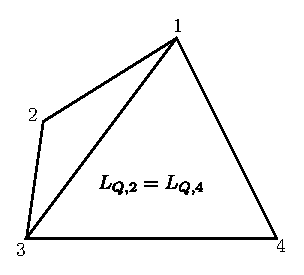
\includegraphics{figures/fig52-11.3.eps}
\caption{}\label{c11:fig11.3}
\end{figure}
$$
L^2_Q = \sum\limits^4_{k=1} \frac{1}{4} \frac{M_Q}{M_k} L^2_{QK}
$$
and
$$
T_Q = \frac{C^2_Q}{S^2_Q} L^2_Q,
$$
where $S_Q$ is the area of $Q$. Then the eigenvalues $\{\mu_\alpha\}$ defined previously obey the inequality.
\begin{equation*}
\mu_\alpha \leq 4 \max\limits_Q . T_Q \tag{11.49}\label{eq11.49}
\end{equation*}
\end{lemma}

\begin{remark}\label{chap11:rem11.3}
The number $S_Q / L_Q$ defines the ``thickness'' of the cell to be used in the Courant-Friedrichs-Lewy condition.
\end{remark}

\begin{remark}\label{chap11:rem11.4}
The bound (\ref{eq11.49}) is quite realistic. In the case of a regular
rectangular mesh, one can compute exactly the $\mu_\alpha, s$ and the
exact bound can be shown to be\pageoriginale 
$$
4 \max \left(\frac{1}{\Delta x^2} , \frac{1}{\Delta y^2}\right). 
$$  
By the lemma the bound appears as
$$
4 \left(\frac{1}{\Delta x^2} + \frac{1}{\Delta y^2}\right). 
$$

These two are generally of the same order.
\end{remark}

Now if $\sum = 0$, we get a necessary and sufficient condition for stability as $\mu_\alpha \Delta t^2 \leq 4$ (which implies that the roots are complex conjugates of each other with modulus 1) or equivalently, 
\begin{equation*}
T^{\frac{1}{2}}_Q \cdot \Delta t \leq 1 \text{ for all } Q. \tag{11.50}\label{eq11.50}
\end{equation*}

If $\sum \neq 0$, but a scalar matrix as above, then we repeat what we did in Sec. \ref{chap9:sec9.6} for the 1-dimensional case and we only give sufficient conditions for the roots to be complex conjugates of each other and for their modulus to be $\leq 1$; namely
\begin{equation*}
\alpha_Q + \beta_{Q/\alpha_Q} \leq 1 \text{ for all } Q\tag{11.51}\label{eq11.51}
\end{equation*}
(hence $\beta_Q \leq \dfrac{1}{4}$), where 
\begin{equation*}
\left. 
\begin{aligned}
\alpha_Q & = \frac{C_Q \Delta t}{(S_Q / L_Q)}\\
\beta_Q  & = \frac{(\sigma_Q)\Delta t}{(S_Q/L_Q)^2} 
\end{aligned}
\right\}
\tag{11.52}\label{eq11.52}
\end{equation*}

Thus again $\beta_Q \leq \dfrac{1}{4}$ resembles the condition for the heat equation. 

For a detailed discussion of stability criteria see Lascaux \cite{key20}.

\section{Concluding Remarks}\label{chap11:sec11.8}

\begin{remark}\label{chap11:rem11.5}
In using\pageoriginale the finite element method for the space discretization we use quadrilateral elements and not triangular elements. We illustrate the difficulties involved when using a triangular mesh by a very particular example.

Consider an incompressible fluid in a square domain where the domain
has been subdivided into $N^2$ equal squares. (Fig. \ref{c11:fig11.4}
(a). One can 
also have a triangular mesh by subdividing each square above into two
triangles by drawing a diagonal of each sqaure. (Fig. \ref{c11:fig11.4} (b)).  

\begin{figure}[H]
\centering
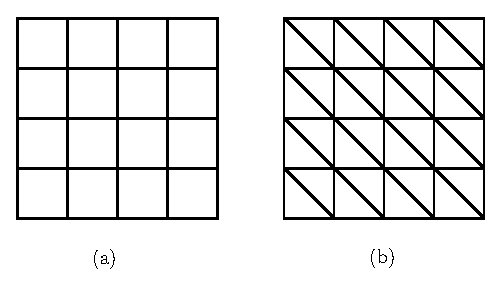
\includegraphics{figures/fig52-11.4.eps}
\caption{}\label{c11:fig11.4}
\end{figure}

In either case we have $(N+1)^2$ nodes and hence computing $u$ and $v$
at these nodes gives $2(N+1)^2$ unknowns. Since the fluid is
incompressible, we get the equation of conservation of mass as 
\begin{equation*}
\text{div}~ \vec{u} = 0\tag{11.53}\label{eq11.53}
\end{equation*}
which is discretised as 
\begin{equation*}
\int\limits_Q ~\text{div}~ \vec{u} dx \; dy = 0 \text{ for all } Q
\tag{11.54}\label{eq11.54} 
\end{equation*}

Since we have $N^2$ squares this gives $N^2$ equations in the first case. However in the second case, we have $2N^2$ equations and then to approximate one equation\pageoriginale alone we have taken up $2N^2$ unknowns out of the available $2 (N^2+1)$. This does not leave many more unknowns for the equation of conservation of momentum.

The finite element method which has been used can be named a `mixed' method because one approximates both the displacements $(x,y)$ and the stresses $(p)$. In order for such a method to work, there must be some compatibility conditions between the corresponding spaces of approximates. (Cf. Raviart, to be published). We have used the space $V_\circ$ for $p,\rho, \epsilon$ and a different space for $\vec{X}$ and $\vec{u}$. For quadrilateral elements we use the space $V_1$ and for triangular elements we have to use another space $V'_1$. It can be shown that the spaces $V_\circ$ and $V'_1$ do not work together while $V_\circ$ and $V_1$ are compatible.

These are some of the reasons for using quadrilateral elements instead of triangular ones.
\end{remark}

\begin{remark}\label{chap11:rem11.6}
  We remarked earlier (Cf. Remark \ref{chap11:rem11.2}) that our mode
  of approximation yielded the 9-point formula for the Laplacian. One
  asks immediately whether ther is a finite element or finite
  difference scheme which gives the {5-point formula} instead. The
  answer is yes. But this is very complicated when using Lagrangian
  variables (Cf. Harlow). In case of the Eulerian variable we have the
  MAC method which has just been devised for this reason. Here
  $p,\rho, \epsilon$ are computed at the centre of each cell while $u$
  is computed at the mid-points of two opposite edges and $v$ at the
  mid-points of the other two edges. (CF. Fig. \ref{c11:fig11.5}). 

\begin{figure}[H]
\centering
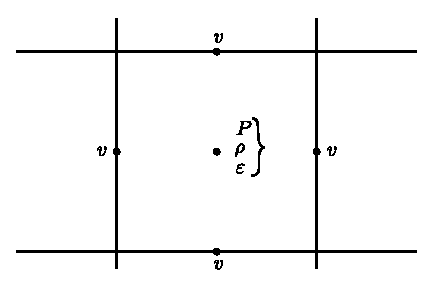
\includegraphics{figures/fig52-11.5.eps}
\caption{}\label{c11:fig11.5}
\end{figure}\pageoriginale 
\end{remark}

\begin{remark}\label{chap11:rem11.7}
Our final comments are on the advantages of the Lagrangian coordinates over the Eulerian coordinates. The principal advantage lies in the tackling of the moving boundary problem or the interface problem. To illustrate how messy the Eulerian equations can become we give an example of an interface between two media.

Given a fixed Eulerian grid, let us examine a cell through which an interface passes and which contains both the media (1 and 2). Then, we must not only know now the boundary moves and where the boundary meets the grid, but also write different equations for the two media. Thus the energy and state equations may be written for the medium $i(i=1,2)$ as
\begin{gather*}
({}^i \epsilon^{n+1} - {}^i \epsilon^n) + \left(\frac{{}^i p^{n+1} +
    {}^ip^n}{2}\right)  \left(\frac{1}{i \rho^{n+1} } - \frac{1}{i
    \rho n }\right) = 0 \tag{11.55}\label{eq11.55}\\ 
  {}^i  \epsilon^{n+1} = f ({}^i p^{n+1}, {}^i \rho^{n+1})
  \tag{11.56}\label{eq11.56} 
\end{gather*}
where the superscript $i$ indicates the medium for which the equations are written. We also have the pressure equality 
\begin{equation*}
{}^1 p^{n+1} = {}^2 p^{n+1}. \tag{11.57}\label{eq11.57}
\end{equation*}\pageoriginale

If Vol.1 and Vol.2 are the volumes occupied by the media and $M_i$ their masses, we have 
\begin{equation*}
\left. 
\begin{aligned}
& M^{n+1}_1 = {}^1 \rho^{n+1}  (\text{Vol.}1)^{n+1}\\
& M^{n+1}_2 = {}^2 \rho^{n+1}  (\text{Vol.}2)^{n+1}\\
& (\text{Vol.}1)^{n+1} + (\text{Vol.}2)^{n+1}  = \text{Vol. of cell } =\\
& \hspace{3.5cm} = \Delta x \Delta y
\end{aligned}
\right\}
\tag{11.58}\label{eq11.58}
\end{equation*}

The equations (\ref{eq11.55}) to (\ref{eq11.58}) are eight in number and there are as many unknowns ($p, \rho, \epsilon$, Vol for each material, assuming $M_1$ and $M_2$ are known) and we must solve such a system.

Moreover the reader is asked to think of how to define the motion of
the interface on the grid and how to provide tests to know when a cell
contains both the media or when it does not. 

A frailty of the Lagrangian method is that when the motion is too
distorted, the quadrilaterals lose their shape and the subsequent
equations will not be meaningful compared to the true situation. In
this regard the ALE method is very useful in two dimensions. One has a
lot of results on this method published by the Los Alamos group
(Harlow et al). The reader is referred to Roache \cite{key33} for its
extensive bibliography where references to these papers can be found. 
\end{remark}

\begin{thebibliography}{99}
\addcontentsline{toc}{chapter}{Bibliography}
\bibitem{key1} ALDER. B., FERNBACH. S., and ROTENBERG,
  M:\pageoriginale  (Editors), \textit{Fundamental Methods in
    Hydrodynamics}. Methods in Computational Physics, Vol. 3, 1964,
  Academic Press, New York. 

\bibitem{key2} AMES, W.F. : \textit{Numerical Methods for Partial
  Differential Equations,} 1969 Barnes and Noble, Inc., New York. 

\bibitem{key3} ARONSON, D.G. : Regularity properties of flows through
  porous media, SIAM Journal of Applied Mathematics, Vol. 17, No. 2,
  1969, pp. 461-467. 

\bibitem{key4} BORIS, J.P. and BOOK, D.L.: Flux Corrected Transport. I
  SHASTA A fluid transport algorithm that works, Journal of
  Comput. Physics Vol. (1973) pp. 38-69. 

\bibitem{key5} BURSTEIN, S.L. and MIRIN, A.A. : Third order difference
  methods for hyperbolic equations, Journal of Computational Physics,
  Vol. 5, 1970, pp. 547-571.  

\bibitem{key6} CIARLET, P.G. : \textit{Lectures on the finite element
  method}, Tata Institute of Fundamental Research, Bombay, 1975. 

\bibitem{key7} CIARLET, P.G. and RAVIART, P.A. : Interpolation theory
  over curved elements with applications to finite elements methods,
  Computer methods in Applied Mechanics and Engineering, Vol. 1, 1972,
  pp. 217-249.  

\bibitem{key8} CONWAY and SMOLLER: Global solutions of the Cauchy
  problem for quasi linear first order equations in several space
  variables, Communications on Pure and Applied Mathematics, Vol. 19,
  1966, pp. 95-105. 

\bibitem{key9} COURANT, R. and FRIEDRICHS, K.O. : \textit{Supersonic
  Flow and Shock Waves}, Interscience, 1948. 

\bibitem{key10} FRIEDRICHS, K.O. : Symmetric positive linear
  differential equations, Communications on Pure and Applied
  Mathematics, Vol. 7, 1958, pp. 333-418.  

\bibitem{key11} FROMM, J.E. : Practical investigation of convection
  difference approximations of reduced dispersion, High Speed
  Computing in Fluid Dynamics - The physics of fluids. Supplement II
  (1969).  

\bibitem{key12} FROMM, J.E. : A method for reducing dispersion
  inconvective difference schemes, Journal of Computational Physics,
  Vol. 3, 1968. pp. 176-189.  

\bibitem{key13} GOURLAY, A.R. and MORRIS, J.L. : One the comparison of
  multistep formulation of the optimized Lax-Wendroff method for
  non-linear hyperbolic systems in two space variables. Journal of
  Computational Physics, Vol. 5. 1970, pp. 229-243.  

\bibitem{key14} GRAVELEAU, J.L. and JAMET, P. :\pageoriginale  A
  finite difference approach to some degenerate non-linear parabolic
  equations, SIAM Journal of Applied Mathematics, Vol.20, No.2, 1971,
  pp. 199-223.  

\bibitem{key15} HIRT, C.W. : Heuristic stability theory for finite
  difference equations, Journal of Computational Physics, Vol.2, 1968,
  pp. 339-355.  

\bibitem{key16} HOSKIN, N.E. : Solution by characteristics of the
  equations of the dimensional unsteady flow, Methods of Computational
  Physics, Vol.3, 1964, pp. 265-294.  

\bibitem{key17} KASAHARA. A. : On certain finite difference methods
  for fluid dynamics, U.S. Monthly Weather Review, Vol.93, No.1,
  January 1965, pp.27-31.  

\bibitem{key18} KOT, C.A. : An improved constant time technique for
  the method of characteristics, \textit{Proceedings of the 3rd
    International Conference in Numerical Methods in Fluid Dynamics,}
  1972, Springer-Verlag, Lecture Notes in Physics.  

\bibitem{key19} KREISS, H.O. : Stability theory for difference
  approximations of mixed initial-boundary value problems - I,
  Mathematics of Computation, Vol.22, No.104, 1968, pp.703-714. 

\bibitem{key20} LASCAUX, P. : Stabilite de la discretisation des
  equations de l'hydrodynamique lagrangienne 2D, A Report, July 1975.  

\bibitem{key21} LAX, P.D. : Weak solutions of non-linear hyperbolic
  equations and their numerical computation, Communications on Pure
  and Applied Mathematics, Vol.7, 1954, pp.159-193. 

\bibitem{key22} LAX, P.D. : Non-linear partial differential equations
  and computing, SIAM Review, Vol.11, No.1, 1969, pp.7-19. 

\bibitem{key23} LAX, P.D. and WENDROFF, B. : Difference schemes with
  high order accuracy for solving hyperbolic equations, Communications
  on Pure and Applied Mathematics. Vol.17, 1964, pp.381.   

\bibitem{key24} LAX, P.D. and WENDROFF, B. : Systems of conservation
  laws, Communications on Pure and Applied Mathematics, Vol.13, 1969,
  pp.217-237. 

\bibitem{key25} LERAT, A. and PEYRET, R. : The problem of spurious
  oscillations in the numerical solution of the equations of gas
  dynamics, \textit{Proceedings of the 4th International Conference on
    Numerical Methods in Fluid Dynamics.} June, 1974, Springer-Verlag,
  Lecture Notes in Physics.  

\bibitem{key26} LIONS, J.L. : \textit{Quelques Methodes de resolution
  de Problemes aux Limites Nonlineaires.} 1969, Dunod, Paris. 

\bibitem{key27} MITCHELL, A.R. : \textit{Computational Methods in
  Partial Differential Equations}, 1969, John Wiley and Sons  

\bibitem{key28} MORTON, K.W. :\pageoriginale Stability and convergence
  in fluid flow problems, Proceedings of the Royal Society, London, A
  323, 1971, pp.237-253.  

\bibitem{key29} NOH, W.F. : \textit{A general theory for the numerical
  solution of the equations of hydrodynamics, Numerical solutions of
  Non-linear Differential Equations} (Ed. D. Greenspan), John Wiley. 

\bibitem{key30} POTTER, D. : \textit{Computational Physics},
  1973. John Wiley and Sons.  

\bibitem{key31} RAVIART. P.-A. : Sur la r\'esolution num\'erique de
  l'\'equation $u_t + u \; u_x - \epsilon (u_x u_x)_x = 0$, Journal of
  Differential Equations, Vol.8, 1970, pp. 56-94. 

\bibitem{key32} RICHTMYER, R.D. and MORTON, K.W. : \textit{Difference
  Methods for Initial Value Problems}, 1967, Interscience Publishers,
  New York.  

\bibitem{key33} ROACHE: \textit{Computational Fluid Dynamics}, Hermosa
  Publishers, Albuquerque.  

\bibitem{key34} ROBERTS, K.V, and WEISS, N.O. : Convective difference
  schemes, Mathematics of Computation, Vol.20. No.94, 1966,
  pp.272-229. 

\bibitem{key35} RUSANOV, V.V. : On difference schemes of third order
  accuracy for non-linear hyperbolic systems, Journal of Computational
  Physics, Vol. 5, 1970, pp. 507-516.  

\bibitem{key36} THOMEE, V. : Stability of difference schemes in the
  maximum norm, Journal of Differential Equations, Vol.1, 1965,
  pp.273-292.  

\bibitem{key37} B. VAN LEER. : Towards the ultimate conservative
  difference scheme. II Monotonicity and conservation combined  in a
  second order scheme Journal of Comput. Physics Vol.14, (1974),
  pp.361-370.  
\end{thebibliography}
